\documentclass[a4paper]{report}
\usepackage[utf8]{inputenc}
\usepackage[portuguese]{babel}
\usepackage{hyperref}
\usepackage{a4wide}
\hypersetup{pdftitle={LI4 - Proposta de Projeto},
pdfauthor={João Teixeira, José Ferreira, Miguel Solino, Maria Silva, Pedro
Oliveira},
colorlinks=true,
urlcolor=blue,
linkcolor=black}
\usepackage{subcaption}
\usepackage[cache=false]{minted}
\usepackage{listings}
\usepackage{booktabs}
\usepackage{multirow}
\usepackage{appendix}
\usepackage{tikz}
\usepackage{authblk}
\usepackage{bashful}
\usepackage{verbatim}
\usepackage{amsmath}
\usepackage{tikz}
\usepackage{tikz,fullpage}
\usepackage{pgfgantt}
\usetikzlibrary{arrows,%
                petri,%
                topaths}%
\usepackage{tkz-berge}
\usetikzlibrary{positioning,automata,decorations.markings}
\AfterEndEnvironment{figure}{\noindent\ignorespaces}
\AfterEndEnvironment{table}{\noindent\ignorespaces}

\begin{document}

\title{LI4 - Proposta de Projeto\\ 
\large PL1 - Grupo 1.1}
\author{José Ferreira (A83683) \and João Teixeira (A85504) \and Maria Silva
(A83840) \and Miguel Solino (A86435) \and Pedro Oliveira (A83762)}
\date{\today}

\begin{center}
    \begin{minipage}{0.75\linewidth}
        \centering
        
\includegraphics[width=0.4\textwidth]{images/eng.jpeg}\par\vspace{1cm}
        \vspace{1.5cm}
        \href{https://www.uminho.pt/PT}
        {\color{black}{\scshape\LARGE Universidade do Minho}} \par
        \vspace{1cm}
        \href{https://www.di.uminho.pt/}
        {\color{black}{\scshape\Large Departamento de Informática}} \par
        \vspace{1.5cm}
        \maketitle
    \end{minipage}
\end{center}

\pagebreak
\chapter{Objetivos atingidos}
Visto que este relatório foi realizado entre entregas apenas alguns dos
objetivos propostos na semana anterior foram realizados. \\
Assim, ao longo desta semana começamos por nos tentar familiarizar com as
tecnologias que vão ser utilizadas para a realização do projeto. Para isso
desenvolvemos um projeto tipo \textit{Hello World} recorrendo a C\#, React e
Neo4J.\\
Em seguida começamos simultaneamente o desenvolvimento da aplicação em React com
a página de login e register e o desenvolvimento do backend em C\#, com a
implementação de classes básicas como o User e o Produto, e inicio da
implementação dos DAOs.

\begin{figure}[H]
    \centering 
    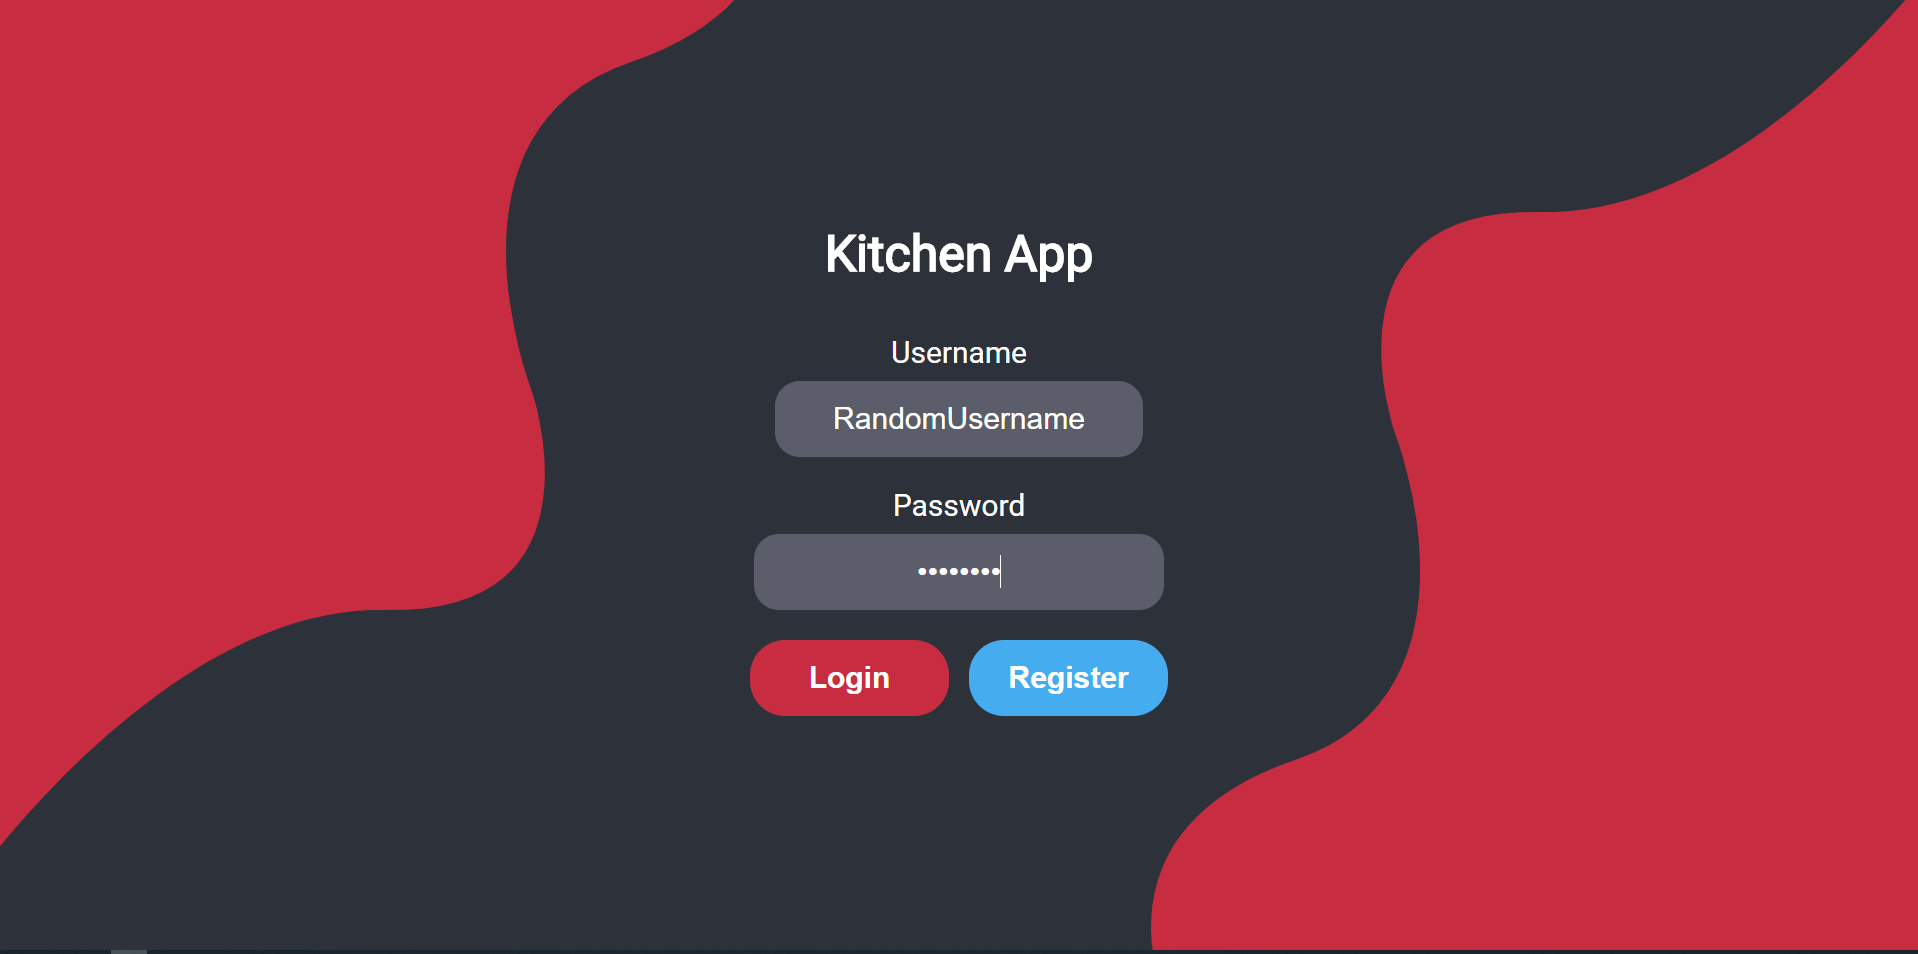
\includegraphics[width=0.5\textwidth]{images/login.png}  
    \caption{login}
    \label{fig:login}
\end{figure}

\begin{figure}[H]
    \centering 
    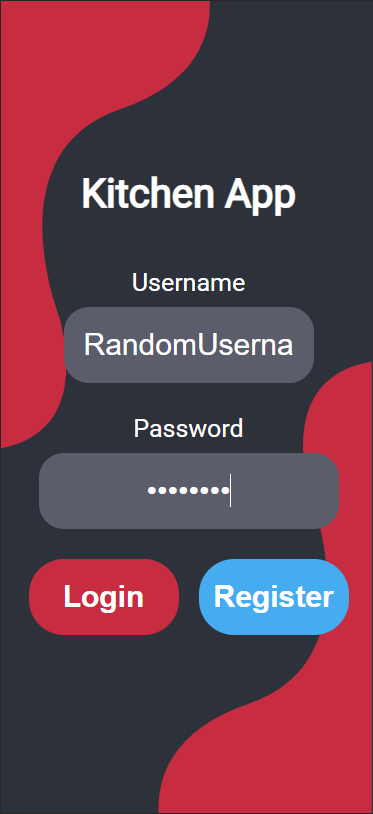
\includegraphics[width=0.2\textwidth]{images/login_mobile.png}  
    \caption{login em mobile}
    \label{fig:login_mobile}
\end{figure}

\begin{figure}[H]
    \centering 
    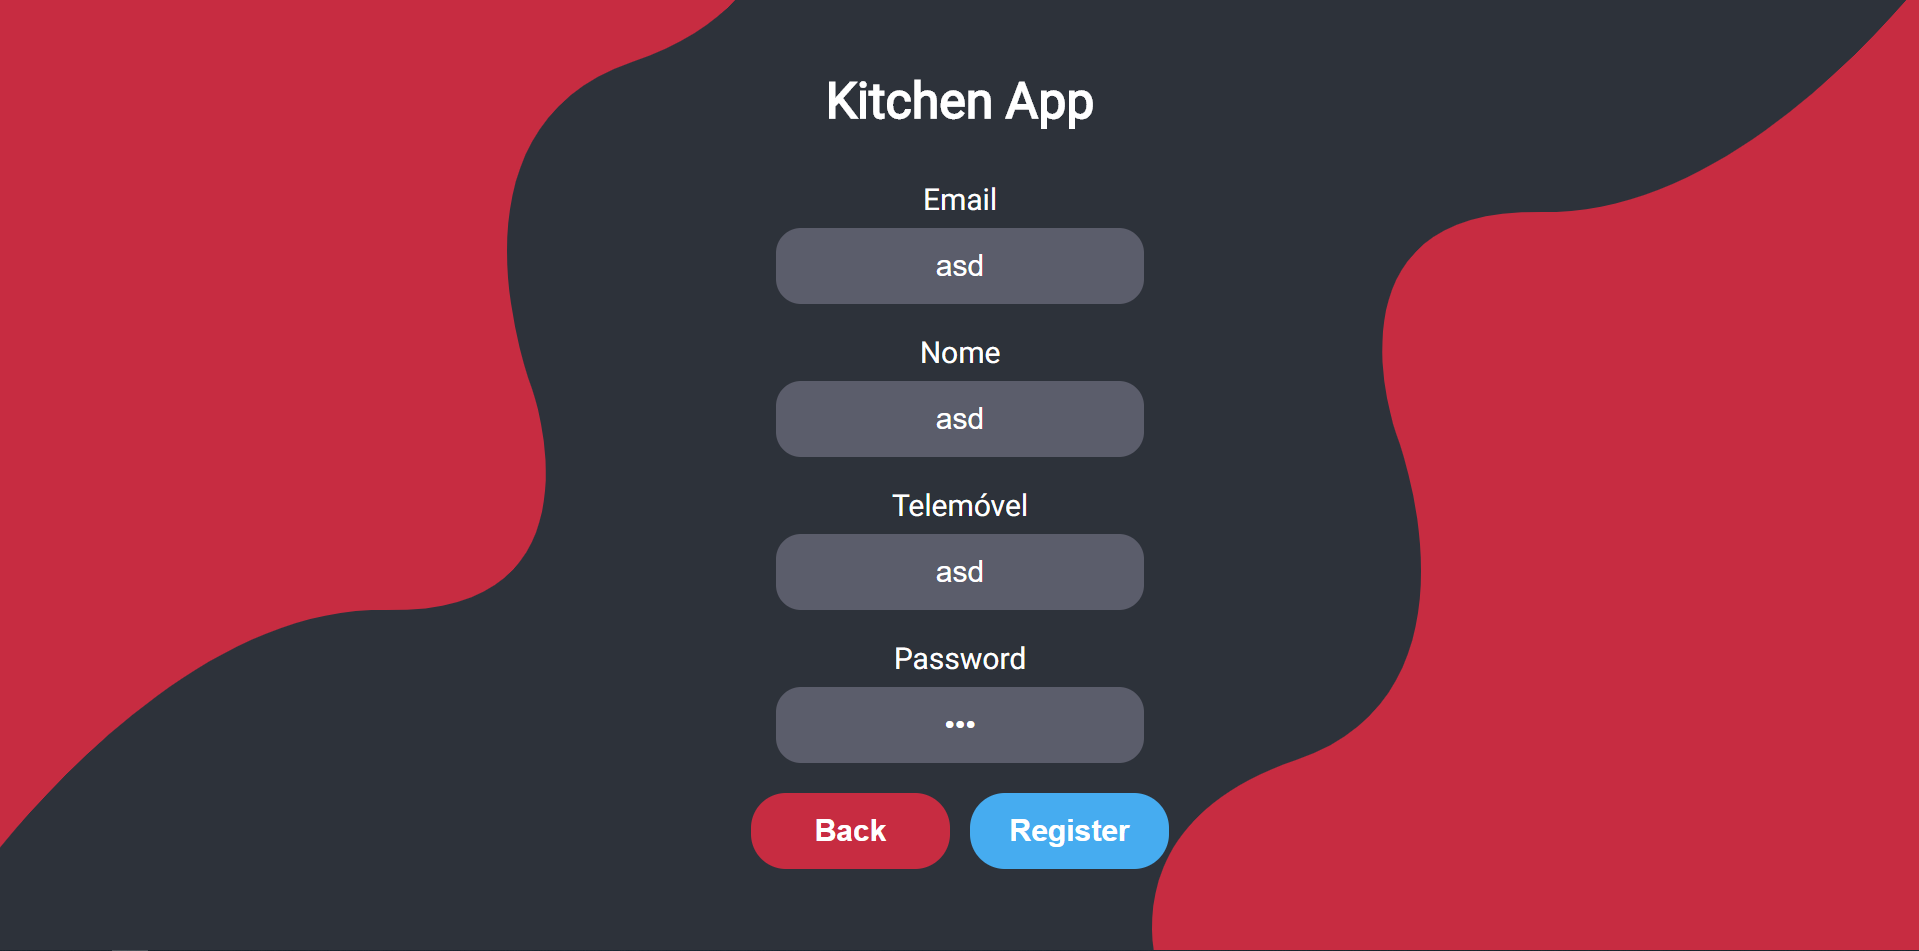
\includegraphics[width=0.7\textwidth]{images/generate.png}  
    \caption{register}
    \label{fig:register}
\end{figure}

\begin{figure}[H]
    \centering 
    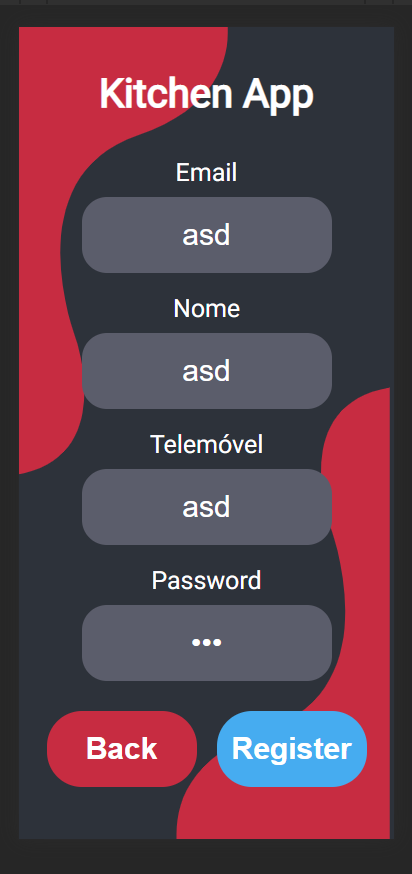
\includegraphics[width=0.3\textwidth]{images/generate_mobile.png}  
    \caption{register em mobile}
    \label{fig:register_mobile}
\end{figure}

\chapter{Objetivos a atingir}
De forma a concluir os objetivos propostos na etapa anterior ao longo da proxim
semana iremos:
\begin{itemize}
    \item Finalização da implementação das classes básicas do backend
    \item Continuar a implementação dos DAOs
    \item Tornar a página de Login e register funcional
    \item Estruturar e popular a base de dados Neo4J com recurso a dados de teste
\end{itemize}

\end{document}
